\subsection{Os modelos conseguem desambiguar adequadamente as sentenças?}\label{resultados-q-3}

Nesta seção, a análise foi baseada nas respostas obtidas na tarefa 3, na qual foi solicitada a desambiguação de todas as sentenças. As respostas obtidas foram divididas em três categorias: 1) Correta ocorreu quando o modelo explica corretamente duas ou mais interpretações possíveis para a sentença, de forma semelhante à interpretação que um ser humano teria. No caso das sentenças sem ambiguidade, o modelo esclarece a ausência de ambiguidade e observa que não é necessário executar a tarefa solicitada; 2) Incompleta ocorreu quando o modelo apresentou pelo menos uma interpretação correta para a sentença, errando nas demais interpretações possíveis; e 3) Incorreta ocorreu quando o modelo apresentou opções de desambiguação sem nenhum sentido. 

Os resultados mostrados na Figura \ref{fig:matriz-confusao-desamb} revelam que ambos os modelos enfrentam dificuldades ao tentar desambiguar corretamente as sentenças, uma vez que propõem interpretações equivocadas, identificando ambiguidade em elementos pouco ou nada relacionados à ambiguidade real. Por exemplo, no conjunto de frases sem ambiguidade, ambos os modelos tentaram desambiguá-las oferecendo opções de interpretação. 

A frase \enquote{\emph{Como o pássaro estava cansado, Ricardo o alimentou.}} obteve uma desambiguação incorreta tanto na tarefa do ChatGPT como do Gemini. No primeiro modelo, a resposta foi a seguinte: \enquote{\emph{Para desambiguar a frase  e torná-la mais clara, podemos reescrevê-la de forma a eliminar a ambiguidade de referência. Uma maneira de fazer isso é substituindo o pronome \enquote{o} por seu referente explícito. Vejamos: 1. Como Ricardo estava cansado, o pássaro foi alimentado por ele. Nesta versão reescrita, fica claro que o pronome \enquote{o} se refere ao pássaro, e não a Ricardo. Agora a frase não possui mais ambiguidade de referência.}} 

O segundo modelo apresentou a seguinte explicação: \enquote{\emph{Claro, aqui estão duas possíveis desambiguações da frase \enquote{Como o pássaro estava cansado, Ricardo o alimentou}: Ricardo alimentou o pássaro porque estava cansado. Ricardo alimentou o pássaro porque estava cansado de ver o pássaro cansado. A primeira interpretação é a mais provável, pois é mais comum alimentar alguém quando está cansado. No entanto, a segunda interpretação também é possível, pois é possível que Ricardo estivesse preocupado com o bem-estar do pássaro e quisesse ajudá-lo a se recuperar. Sem mais informações, não é possível dizer com certeza qual é a interpretação correta.}}

Os modelos desambiguaram sem necessidade mais de 90\% dos casos de teste do conjunto de frases sem ambiguidade. É relevante destacar que, mesmo o ChatGPT - que afirmou em perguntas anteriores que algumas frases não tinham ambiguidade - ofereceu opções de desambiguação, sendo incongruente com suas respostas anteriores. Uma exceção notável ocorreu em uma resposta relacionada à frase \enquote{Gostamos da cor rosa}, na qual o ChatGPT afirmou: \enquote{\emph{Peço desculpas, mas a frase 'Gostamos da cor rosa' não é intrinsecamente ambígua e, portanto, não requer desambiguação. Ela expressa claramente uma preferência pela cor rosa. Se houver um contexto específico causando ambiguidade, por favor, forneça mais informações para que eu possa ajudar a esclarecer a situação}}. Observa-se que os modelos têm a tendência de realizar superinterpretações das sentenças sem ambiguidade, oferecendo soluções sem lógica apenas para cumprir a tarefa solicitada, demonstrando ainda não haver o conhecimento explícito de regras do funcionamento da língua.

%\begin{table}[h]
%\caption{Estatísticas obtidas na tarefa de desambiguação.}
%\label{tab:estat_desambiguacao}
%\begin{tabular}{lcccccc}
%\hline
%Grupo                 & \multicolumn{2}{c}{Corretas} & \multicolumn{2}{c}%{Incompletas} & \multicolumn{2}{c}{Incorretas} \\ \hline
%                      & ChatGPT        & BARD        & ChatGPT          & BARD         & ChatGPT         & BARD         \\
%Sem ambiguidade       & 12               & 3            & 0                 & 6             & 108                & 108             \\
%Ambiguidade Sintática & 15             & 20              & 19               & 13             & 6               & 7              \\
%Ambiguidade Semântica & 31               & 23              & 3                 & 3             & 6                & 14             \\
%Ambiguidade Lexical   & 28               & 29             & 7                 & 5           & 5                 & 6              \\ \hline
%\end{tabular}
%\source{Própria.}
%\notes{Se necessário, poderá ser adicionada uma nota ao final da tabela.}
%\end{table}


\begin{figure}[htb]
    \centering
    \begin{subfigure}[b]{0.45\textwidth}
        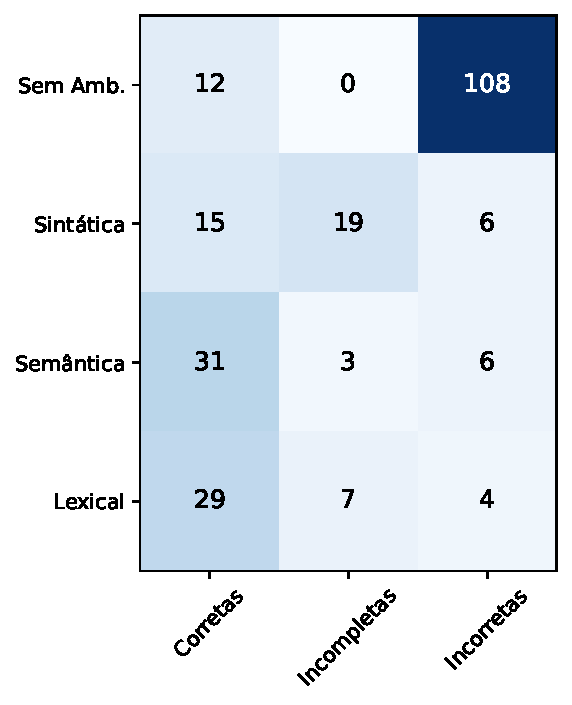
\includegraphics[width=\textwidth]{matriz_confusao_desamb_ChatGPT.pdf}
        \caption{Resultados quantitativos da tarefa de desambiguação realizada pelo ChatGPT.}
        \label{fig:matriz_confusao_chatgpt}
    \end{subfigure}
    \hfill
    \begin{subfigure}[b]{0.45\textwidth}
        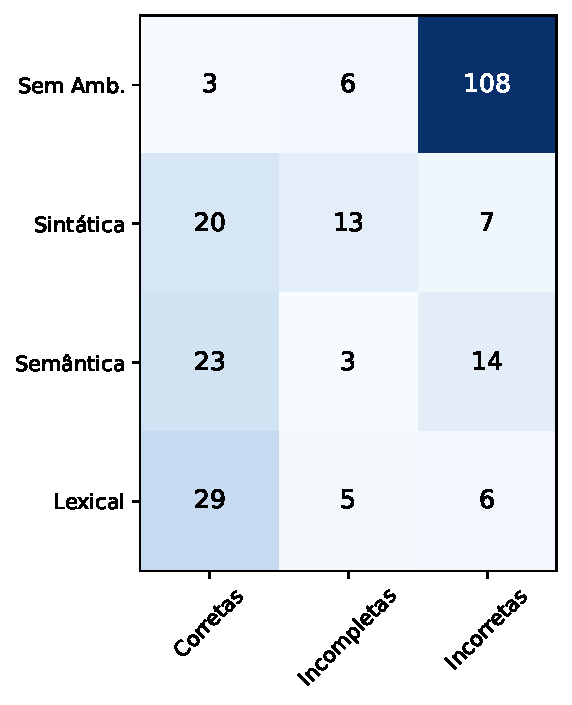
\includegraphics[width=\textwidth]{matriz_confusao_desamb_Bard.pdf}
        \caption{Resultados quantitativos da tarefa de desambiguação realizada pelo Gemini.}
        \label{fig:matriz_confusao_bard}
    \end{subfigure}
    \caption{Estatísticas obtidas na tarefa de desambiguação. Os resultados mostram que ambos os modelos apresentam muita dificuldade para identificar que as sentenças distratoras não tem ambiguidade. Em 108 casos de teste, ambos os modelos forneceram explicações que não refletiam a interpretação humana, justificando a presença de ambiguidade em sentenças que, na verdade, não a possuíam.}
    \label{fig:matriz-confusao-desamb}
\end{figure}



Na desambiguação das frases com ambiguidade sintática, os modelos também apresentaram erros na maioria dos testes. Em 62,5\% dos testes, as análises apresentadas estavam incorretas ou incompletas e os critérios usados nas frases classificadas com ambiguidade sintática, também, pendiam para uma abordagem semântica, lexical ou voltada para a necessidade de um contexto favorável para desambiguar as sentenças. No caso da sentença \enquote{Pedro me mandou um cartão postal de Veneza}, o ChatGPT apresentou a seguinte desambiguação para a frase: \enquote{Pedro me mandou um cartão postal de Veneza}; \enquote{Pedro mandou um cartão postal de Veneza para a minha amiga Maria, e ela me mostrou o cartão}. Contudo, a ambiguidade no adjunto \enquote{de Veneza} permanece. Outra solução proposta é mudar a alocação do pronome: \enquote{Pedro mandou um cartão postal de Veneza para mim}, mantendo a frase ambígua. Nesse caso, o Gemini ofereceu melhores opções, como \enquote{Pedro está atualmente em Veneza e me enviou um cartão postal que foi produzido lá.} ou \enquote{Pedro não está atualmente em Veneza, mas me enviou um cartão postal que mostra uma imagem da cidade.},  demonstrando aplicar os princípios da aposição mínima e da aposição local \cite{maiadimensoes} para resolver a ambiguidade. No entanto, o modelo, na maioria das vezes, não conseguiu identificar com precisão qual era o elemento causador da ambiguidade.

Por outro lado, no grupo de frases com ambiguidade semântica, na maior parte dos testes, ambos os modelos de linguagem sugeriram frases adequadas para a desambiguação das sentenças, sempre destacando a importância do contexto para a correta interpretação. Um exemplo pode ser visto com a frase \enquote{Ana me contou um segredo sobre ela}, em que o ChatGPT propôs a desambiguação esperada, compreendendo que \enquote{ela} pode se referir tanto à Ana, quanto a uma outra pessoa. Em relação às respostas do Gemini, a maioria também foi apropriada porém com precisão menor que a ChatGPT. Por exemplo, em \enquote{Paulo não entrou na universidade de novo}, o Gemini indicou corretamente que as possíveis reescritas da sentença seriam \enquote{Paulo não foi aceito na universidade de novo} e \enquote{Paulo não entrou na universidade de novo depois de ter se formado}. Já em \enquote{A carteira foi danificada}, o Gemini sugeriu opções que especificassem informações não necessariamente ambíguas, visto que ele interpretou que a ambiguidade estaria em \enquote{danificado}, assim, deveria ser especificado se \enquote{A carteira foi danificada fisicamente} ou \enquote{A carteira foi danificada financeiramente}. Estas interpretações são bastante distantes do que se encontra em estudos psicolinguísticos sobre processamento \cite{machado1996sintaxe, brito2013processamento}.

Os modelos tiveram, simultaneamente, melhor desempenho nos casos de ambiguidade lexical (Figura \ref{fig:matriz-confusao-desamb}), entretanto, o ChatGPT não conseguiu desambiguar corretamente algumas frases que envolvem polissemia. Na frase \enquote{Pedi um prato ao garçom.}, o modelo apresentou duas opções de desambiguação com a seguinte resposta à tarefa 3: \enquote{Claro, aqui estão as duas possíveis interpretações desambiguadas da frase:  Eu pedi um prato ao garçom.  Eu pedi ao garçom um prato. Essas reestruturações eliminam a ambiguidade, deixando claro quem realizou a ação de pedir e o que foi pedido.}. Percebe-se, então, que o modelo tende a encontrar problemas na estrutura, ao trocar a posição dos elementos sintáticos e não nas palavras isoladamente. O Gemini apresentou mais facilidade de identificação e explicação nos casos de homonímias, haja vista que todas as suas explicações nestes casos estão corretas. Por outro lado, também predominaram justificativas equivocadas em alguns casos de polissemia.
